\chapter{Fringing}
\label{sec:fringe}

\textit{The problem.} Beyond $\approx6500$\,\AA{} the FLOYDS red order shows fringes: an interference pattern of the
CCD that modulates the spectrum by up to 10--20 per cent with a period of $\approx38$\,\AA{}
(see the Conventions, p.~\pageref{sec:conventions}). Because reverberation mapping compares spectra taken on different nights, the
fringes must be removed from every single spectrum, not only on average.

\textit{What the archive does.} \banzai{}~1.0.1 divides each 2-d frame by a whole lamp flat taken months earlier,
shifted along the slit by a fitted offset. This removes the fringes poorly, imprints the lamp's own illumination
pattern on the science, and in some frames destroys pixels (Section~\ref{sec:fringe_banzai}).

\textit{What we changed.} The frame is no longer divided by a flat. Instead, the fringes are fitted in each extracted
1-d spectrum with a \emph{harmonic model}: a sum of sine waves whose phase is taken from the lamp flats and whose
amplitude and shape are fitted to the spectrum itself (Section~\ref{sec:fringe_harmonic}). Inside the pipeline the
model was then refined in the 6500--7500\,\AA{} region and fitted jointly with the telluric absorption
(Sections~\ref{sec:fringe_pipeline} and \ref{sec:fringe_joint}).

\textit{How much better.} The fringe metric of Table~\ref{tab:summary} (the rms of the ratio of 25 and 200\,\AA{}
running medians in the telluric-free windows 7750--8050 and 8450--8900\,\AA) of the Fairall~9 spectra drops from 13.7
per cent in the archive and 8.1 per cent in \banzai{}~1.1.0 to 1.9 per cent in improved v3
(Table~\ref{tab:versions}). In this chapter, names in typewriter font are the corresponding \banzai{} settings,
header keywords or scripts, given for readers who want to reproduce the results.

\section{What \banzai{}~1.0.1 does}
\label{sec:fringe_banzai}
Each archive \texttt{-2d} product stores, in its \texttt{FRINGE} extension, the map $\Phi(x,y)$ by which
\banzai{}~1.0.1 divided the frame. Inspecting these maps, we find four problems:
\begin{enumerate}
\item $\Phi$ is a whole normalised lamp flat (taken 2026 March 14/15, eight months before the science), not only its
fringe component. Besides the fringes it contains the lamp's illumination profile along the slit (bands of
$\pm5$ per cent at 5000--7000\,\AA) and flat-field structure. It is applied from $\approx5000$\,\AA{}
(Fig.~\ref{fig:master}).
\item The map is shifted \emph{along the slit} by an offset fitted to each frame (header keyword
\texttt{L1FRNGOF}). Cross-correlating the maps of two frames gives a shift equal to the difference of their offsets
(17 rows for offsets $+9.0$ and $-8.5$). The fitted offsets range from $-575$ to $+182$\,pixels and cluster near
$\pm9$ and $\pm14$\,pixels, where the periodic fringe pattern gives false matches; the real flexure is only
1--2\,pixels.
\item Where the shifted map has no data (rows shifted in from beyond the edge of the flat), it holds either
quantisation noise ($\sim10^{-6}$) or values up to $\pm3\times10^4$. In 13 of the 50 Fairall~9 frames (all with
offsets between $-8.5$ and $-11.1$) this invalid edge falls inside the illuminated order at 5200--5700\,\AA{}. The
pixels there are divided by values $\gg1$, the 2-d sky model oscillates into stripes, and the extraction turns these
into 25--127 spikes per spectrum (Fig.~\ref{fig:edge}).
\item Because the whole flat is used, every frame is divided by the lamp's illumination profile at the rows where the
object lies. This is a factor of up to $\pm10$ per cent that depends on the frame and on wavelength (a 15 per cent
excess at 5500--7000\,\AA{} in a bright-moon frame).
\end{enumerate}

\begin{figure}[!htbp]
\centering
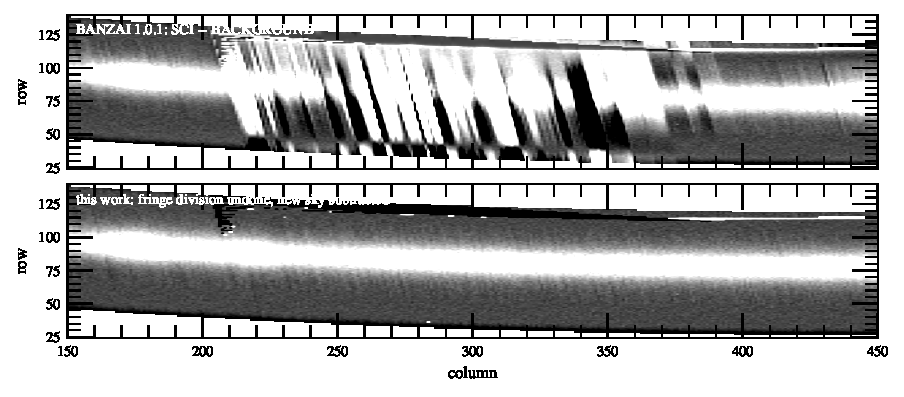
\includegraphics[width=\textwidth]{figures/fig_edge.pdf}
\caption{Red order at $\approx5000$--6000\,\AA{} of the bright-moon frame 2026-10-26 \#13. Top: archive SCI minus
BACKGROUND. Bottom: improved v1 (fringe division undone, invalid pixels masked, new sky subtracted; Appendix~\ref{sec:app_v1}).}
\label{fig:edge}
\end{figure}





\section{Harmonic fringe model}
\label{sec:fringe_harmonic}
\banzai{}~1.1.0, run from the raw frames, no longer divides the frame by the lamp flat. In our reductions from the
raw frames (improved v2 and v3) the fringes are removed from the extracted spectrum with the model of this section. The model was first developed on the archive
products (improved v1), where the 1.0.1 division had to be undone first (Appendix~\ref{sec:app_v1}). In both cases
the input is the fringe component $\delta$ of a lamp-flat pattern: the lamp flat divided by its running median along
the dispersion, which keeps only the fringes. In the pipeline the pattern is the median of the processed lamp flats
of one slit width over one to two months (the phase master, Section~\ref{sec:fringe_pipeline}); for the archive
products it is given by eq.~(\ref{eq:delta}).

\textit{Why a scaled lamp pattern cannot work.} The simplest correction, used in our first version (improved v1),
divides the spectrum by the lamp's fringe pattern multiplied by an amplitude $A(\lambda)$ calibrated per slit width
(the \emph{amplitude law}, Appendix~\ref{sec:app_v1}). Fig.~\ref{fig:harmonic} shows why this is not enough. It
shows the red order of a standard and of a Fairall~9 frame before fringe correction, divided by a smooth continuum.
The fringes have sharp maxima and broad, shallow minima, as expected from the Fabry--P\'erot transmission of the
thinned CCD. The scaled lamp pattern is almost sinusoidal. When its maxima match the data, its minima are too deep
(normalised minima of 0.55--0.6 instead of 0.75--0.8), which produces the asymmetric, spiky residuals of the
amplitude-law correction.

The reason is the range of wavelengths that reaches each pixel. A pixel at column $x$ receives the wavelength
$\lambda_0(x)-D\,s$ from every illuminated position $s$ across the slit, with $D$ the dispersion. The recorded fringe
is therefore the CCD transmission $\mathcal{T}(x,y,\lambda)$ smoothed by the image of the light across the slit, in
wavelength units. For the lamp, which fills the slit, this kernel is a top-hat of the slit width (51\,\AA{} in the red
order for the 6\,arcsec slit, larger than the $\approx38$\,\AA{} fringe period); for a point source it is the seeing
profile. If $\mathcal{T}$ is written locally as a Fourier series in its phase $\phi$, harmonic $k$ is multiplied by
the Fourier transform of the kernel at $k$ times the fringe frequency. A symmetric kernel preserves the phase. The
slit-filling lamp, however, suppresses the fundamental and, much more, the harmonics, by factors that depend on
wavelength (the period grows as $\lambda^2$) and differ from those of the object. The lamp flat therefore gives the
\emph{phase} of the fringes but neither their amplitude nor their shape. In addition, the object's phase is offset
from the lamp's by flexure and by its position across the wide slit, both of which change the wavelength falling on
each pixel: a 5\,\AA{} offset moves the phase by $\approx0.2$ cycles. The free fits below give a frame-to-frame phase scatter of 16--26$^\circ$ for Fairall~9 and
6--9$^\circ$ for EG\,21; a 20$^\circ$ error alone leaves a residual of $2\sin(10^\circ)A\approx0.35A$, about a third of the
fringe amplitude.

\begin{figure}[!htbp]
\centering
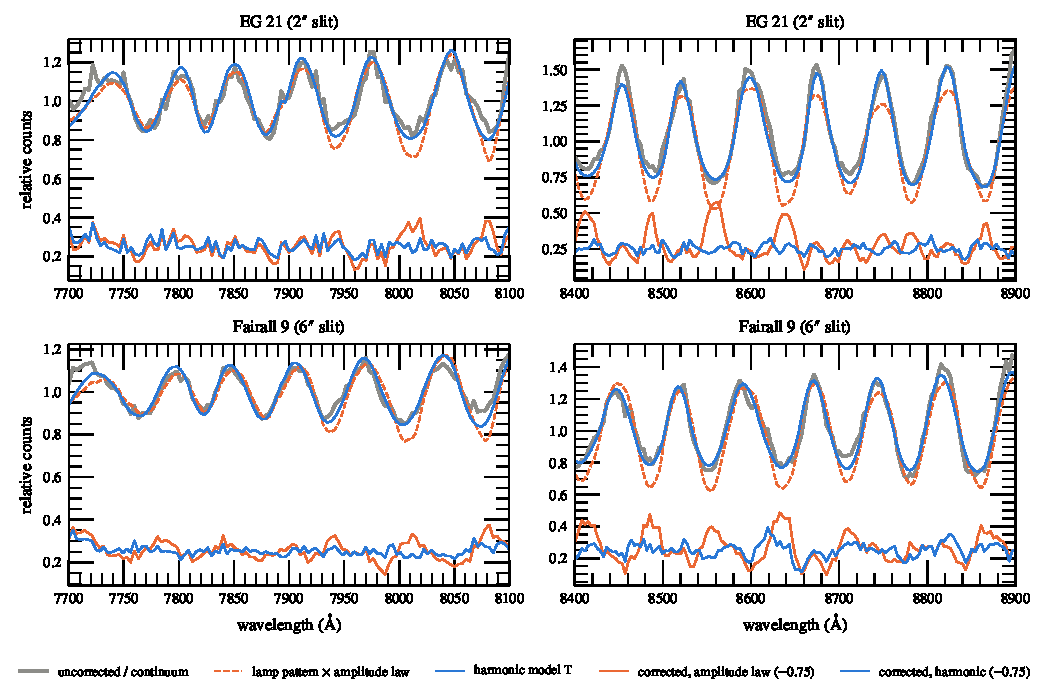
\includegraphics[width=\textwidth]{figures/fig_harmonic.pdf}
\caption{Fringe shape at 8400--8900\,\AA{} in the red order of an EG\,21 frame (left) and a Fairall~9 frame (right).
Top: the extraction before fringe correction over its 150\,\AA{} running median (grey), the lamp pattern times the
amplitude law (dashed; its minima are too deep) and the harmonic model $T$ (eq.~\ref{eq:harmonic}). Bottom: the
spectrum corrected with each model, over its running median; the rms in this window is given above each panel.}
\label{fig:harmonic}
\end{figure}


\textit{Phase map.} For every row of the red order, we take the fringe phase from the lamp-flat fringe component,
smoothed with a Gaussian of $\sigma=1$ pixel, as the argument of its analytic signal:
\begin{equation}
\phi(x,y)=\arg\left\{\tilde\delta(x,y)+i\,\mathcal{Q}_x[\tilde\delta](x,y)\right\},
\label{eq:phase}
\end{equation}
where $\mathcal{Q}_x$ is the Hilbert transform along the dispersion and $\tilde\delta$ the smoothed $\delta$ (eq.~\ref{eq:delta}).

\textit{Model and fit.} The fringe transmission $T(\lambda)$ of the extracted spectrum (the factor by which the
fringes multiply it) is modelled in logarithm as
\begin{equation}
\ln T(\lambda)=\sum_{k=1}^{K}\sum_{j=1}^{J}h_j(\lambda)\left[a_{jk}\,C_{k,\beta}+b_{jk}\,S_{k,\beta}\right],
\label{eq:harmonic}
\end{equation}
\begin{equation}
C_{k,\beta}=\frac{\sum_{i\in\beta}P_iw_i\cos k\phi_i}{\sum_{i\in\beta}P_i},
\label{eq:harmproj}
\end{equation}
Here $\beta$ is a 1-pixel wavelength bin of the extracted spectrum and $i$ runs over the 2-d pixels in that bin, with
phase $\phi_i$ and profile weight $P_i$ (the fraction of the object's light in pixel $i$). $C_{k,\beta}$ is thus the
profile-weighted mean of $\cos k\phi$ in the bin, and $S_{k,\beta}$ is defined likewise with $\sin k\phi_i$. $w_i$ is
the taper of eq.~(\ref{eq:delta}), which switches the model on gradually at the blue end. The $h_j$ are linear
interpolation functions on the nodes $\lambda_j=6800,7300,\dots,9800$\,\AA{} ($J=7$), so the coefficients
$a_{jk},b_{jk}$ are allowed to vary smoothly with wavelength. $k$ is the harmonic number; we use $K=2$
(28 coefficients), and $K=1$ is only slightly worse. The $b_{jk}$ absorb the phase offset of the frame, and the
$a_{jk}$ and $b_{jk}$ together give the amplitude and shape of the fringes. The coefficients are the linear
least-squares solution of
\begin{equation}
\mathcal{H}_{150}[\ln F_\beta]=\sum_{j,k}a_{jk}\,\mathcal{H}_{150}[h_jC_k]_\beta+b_{jk}\,\mathcal{H}_{150}[h_jS_k]_\beta,
\label{eq:harmfit}
\end{equation}
where $F$ is the extraction without fringe correction and $\mathcal{H}_{150}$ subtracts a 150\,\AA{} running median.
The fit uses three iterations of $5\sigma$ clipping. The telluric bands need care. If they are simply excluded,
the coefficients across 8900--9300\,\AA{} are constrained only by the neighbouring regions, and the residual there
is 8--9.5 per cent. The fit is therefore done in two passes. The first excludes
the bands (6860--6960, 7150--7350, 7560--7720, 8100--8380 and 8900--9300\,\AA) and is followed by the wavelength and
flux calibration, which yield the telluric transmission $t$ of each spectrum (Section~\ref{sec:flux_tell}); the second
refits eq.~(\ref{eq:harmfit}) on $F/t$, excluding only the A band and pixels with $t<0.3$. In a test on all frames this
lowers the residual at 8950--9300\,\AA{} from 8--9.5 to 5.3--5.6 per cent and at 9300--9700\,\AA{} from 8.2--8.5 to
6.8--8.5 per cent, with the residual in the clean windows unchanged. The extracted counts and their
uncertainties (both the optimal and the fixed-aperture extraction) are then divided by $T$. The fit uses only the
frame's own spectrum and the phase map, and no information on the target. Because the basis oscillates with the fringe phase, it is nearly orthogonal to
astrophysical structure on scales above $\approx50$\,\AA, and the clipping removes narrow features.

\textit{Variants tested} (Table~\ref{tab:fringevariants}). (i) The phase can be taken from the eight-month-old
master pattern recovered from the archive maps (Appendix~\ref{sec:app_v1}), or from the lamp flat taken in the same
block as each science frame (69 such flats exist for the Fairall~9 campaign, matched by block identifier; command-line
option \texttt{--flat-dir}). Their fringe components correlate with the master at $r=0.95$--0.98, and the harmonic
correction with same-block phases is indistinguishable from the one with the master. The detector pattern is stable
over the eight months, so the age of the flat was not the limiting factor. (ii) The classical approach measures the
fringes on a standard star and transfers them to the science frame. Here we used the high-passed $\ln F$ of the
nearest EG\,21 spectrum, with a free shift and a free scale at each node. It does better than the amplitude law but
worse than the harmonic model, because the phase offset differs between exposures. (iii) For the AGN, fixing the
harmonic coefficients to their median over all frames, or fixing only the amplitude and fitting the phase, is worse
than fitting all coefficients freely in each frame.

\begin{table}
\centering
\caption{Fringe residuals of the red order: rms of $\ln F$ after subtracting a 150\,\AA{} running median, in
7750--8050 and 8450--8900\,\AA, per cent, median over frames. No short smoothing is applied, so photon noise sets a
floor (last row). $^{a}$16 frames with a lamp flat within one day.}
\label{tab:fringevariants}
\begin{tabular}{lcc}
\toprule
Correction & Fairall~9 & EG\,21 \\
 & (\%) & (\%) \\
\midrule
None & \FVnoneF & \FVnoneE \\
Amplitude law (master pattern) & \FVampF & \FVampE \\
Standard-star transfer & \FVstdF & -- \\
Harmonic, ensemble coefficients & \FVensF & \FVensE \\
Harmonic, master phase & \FVharmF & \FVharmE \\
Harmonic, same-block flat phase & \FVflatF & \FVflatE$^{a}$ \\
Photon-noise floor & \FVnoiseF & \FVnoiseE \\
\bottomrule
\end{tabular}
\end{table}

\section{The harmonic model inside the pipeline, and the 6500--7500\,\AA{} region}
\label{sec:fringe_pipeline}
In the reduction from the raw frames (Chapter~\ref{sec:raw}) the frame is never divided by a lamp flat (setting
\texttt{FRINGE\_METHOD = 'harmonic'}). Instead, a new pipeline stage, \texttt{HarmonicFringeCorrector}, fits
eq.~\ref{eq:harmonic} to each extracted spectrum, after the telluric transmission of the standard has been loaded.
The initial configuration used the settings developed on the archive products: phase from the lamp flat of the same
block, model tapered in from 6500\,\AA{} and fully on at 6800\,\AA, amplitude nodes every 500\,\AA{} from
6800\,\AA, and fit on the telluric-corrected spectrum. It matched the archive-based recalibration (improved v1)
redward of 7700\,\AA, but residual fringes were visible at 6500--7500\,\AA{} in the individual Fairall~9 spectra.

We tested twelve variants offline on all 157 frames reduced from the raw data. For each variant, the uncorrected
extraction of each frame was refitted and scored. The stars were scored by the rms of the 12/150\,\AA{} high-pass
(see the Conventions, p.~\pageref{sec:conventions}) in windows free of lines and telluric bands. Fairall~9 has no line-free windows at
these wavelengths, so it was scored by the scatter between its 100 spectra; this measures only the frame-specific
part of the residual, since fringes common to all frames cancel. Table~\ref{tab:fringebench} summarises the result:
\begin{enumerate}
\item Below 6450\,\AA{} the fringes are $\lesssim0.3$ per cent. Starting the model at 5800\,\AA{} only adds noise
(Fairall~9 at 6000--6450\,\AA: 0.93$\rightarrow$1.16 per cent), so the onset stays at 6500\,\AA.
\item The phase of a single 6\,arcsec lamp flat is noisy at 6500--7500\,\AA, where the lamp fringes have little
contrast. The per-frame fit then injects bumps that differ from frame to frame (Fairall~9 at 6450--6850\,\AA:
1.34 per cent, against 0.94 uncorrected). A phase master, the median of the fringe patterns of all lamp flats of one
slit width over one to two months, removes most of this.
\item Fitting on the telluric-corrected spectrum transfers the residuals of the standard's telluric transmission
(Chapter~\ref{sec:flux}) into the fringe model. Masking all telluric bands is better everywhere except redward of
the 8900\,\AA{} water band, where there is no telluric-free stretch left.
\item The phase was taken from the Hilbert transform of the lamp pattern smoothed by one pixel (eq.~\ref{eq:phase}).
But the pattern also contains slow structure: the slit illumination and the shape of the lamp spectrum, 4--5 per cent
rms even at 6000--6500\,\AA{} where there are no fringes. Where the fringe contrast is low, at 6500--7500\,\AA{}
through a wide slit, this slow structure sets the phase, and the fit removes almost nothing: in the individual
Fairall~9 spectra the fringes at 7100--7550\,\AA{} were nearly unchanged by the correction. Removing structure longer
than 31\,px with a running median before the Hilbert transform fixes this. The fringe period grows from
$\approx8$\,px at 7000\,\AA{} to 15--20\,px beyond 8500\,\AA, where a 31\,px filter would affect the fringes
themselves. We therefore use this high-passed phase blueward of 7600\,\AA{} and the plain phase redward of
7900\,\AA, interpolating between the two angles in between (setting \texttt{FRINGE\_PHASE\_HIGHPASS}). On Fairall~9
the rms of the high-passed spectra at 6960--7150\,\AA{} drops from 1.13 to 0.90 per cent (uncorrected 1.37). At
7350--7550\,\AA{} it drops from 3.75 to 3.44 per cent (uncorrected 4.53; He\,{\sc i}\,7065 and
[Ar\,{\sc iii}]\,7136 fall in this window). The stars are unchanged.
\item More harmonics, more phase smoothing or a fixed high-pass at all wavelengths do not help.
\end{enumerate}
The configuration at this stage (improved v2, last row of Table~\ref{tab:fringebench}) used the phase master
(setting \texttt{FRINGE\_PHASE\_SOURCE = 'stacked'}) with the blended high-pass phase, nodes every 400\,\AA{} from
6600\,\AA, and all telluric bands masked. Redward of the 8900\,\AA{} water band, where no band-free stretch is left,
it switches to a fit on the telluric-corrected spectrum, blending the two fits between 8850 and 8950\,\AA{} (setting
\texttt{FRINGE\_TELLURIC\_BLEND}). Both fits are small linear least-squares problems.

\begin{table}[!htbp]
\centering
\small
\caption{Fringe-model variants on the 157 frames reduced from raw. Stars (EG\,21, Feige\,110): median rms (per cent)
of a 12/150\,\AA{} high-pass in line- and telluric-free windows. Fairall~9: small-scale scatter between the
spectra (per cent; frame-specific part only).}
\label{tab:fringebench}
\footnotesize
\setlength{\tabcolsep}{3.2pt}
\begin{tabular}{@{}>{\raggedright\arraybackslash}p{3.7cm}ccccc|ccccc@{}}
\toprule
 & \multicolumn{5}{c|}{Stars: window (\AA)} & \multicolumn{5}{c}{Fairall~9: window (\AA)} \\
 & 6650-- & 6960-- & 7350-- & 7750-- & 8450-- & 6000-- & 6450-- & 6950-- & 7700-- & 8500-- \\
Variant & 6850 & 7150 & 7550 & 8050 & 8900 & 6450 & 6850 & 7550 & 8500 & 9200 \\
 & (\%) & (\%) & (\%) & (\%) & (\%) & (\%) & (\%) & (\%) & (\%) & (\%) \\
\midrule
uncorrected & 1.73 & 3.64 & 5.43 & 11.39 & 26.49 & 0.92 & 0.94 & 1.80 & 3.24 & 4.42 \\
initial configuration & 0.73 & 1.18 & 1.12 & 2.04 & 4.76 & 0.93 & 1.34 & 1.91 & 2.52 & 3.37 \\
onset 5800\,\AA, nodes 400\,\AA & 0.69 & 1.23 & 1.24 & 2.10 & 4.83 & 1.16 & 1.31 & 1.81 & 2.45 & 3.34 \\
\quad + phase master & 0.70 & 1.19 & 1.24 & 2.13 & 4.82 & 1.01 & 1.21 & 1.68 & 2.35 & 3.34 \\
\quad + all bands masked & 0.56 & 1.08 & 1.27 & 1.52 & 3.12 & 1.18 & 1.18 & 1.85 & 2.25 & 4.21 \\
phase master, all bands masked, nodes 400\,\AA{} from 6600 & 0.60 & 1.11 & 0.92 & 1.55 & 2.89 & 0.92 & 1.02 & 1.79 & 2.29 & 3.60 \\
\quad + telluric-corrected fit beyond 8850\,\AA & 0.59 & 1.11 & 0.92 & 1.49 & 2.99 & 0.92 & 1.05 & 1.77 & 2.29 & 3.27 \\
\quad + phase high-pass 31\,px blueward of 7600\,\AA{} (improved v2) & 0.66 & 1.08 & 0.99 & 1.57 & 2.99 & 0.90 & 0.98 & 1.56 & 2.24 & 3.27 \\
\bottomrule
\end{tabular}
\end{table}

\subsection{Joint telluric fit, earlier onset, denser nodes and a residual template}
\label{sec:fringe_joint}
Two problems remained with that configuration.
(i) Inside the water bands (7170--7330 and 8130--8360\,\AA) the Fairall~9 spectra kept 4 per cent rms of structure on
fringe scales (12/150\,\AA{} high-pass), against 1.7--3.2 per cent in the archive-based recalibration (improved v1).
Most of it (3.1 per cent) was common to all spectra. With the bands masked, the fringes inside them are only
interpolated from the band edges. The residual therefore stays in the transmission measured on the standards and,
through the telluric correction with the median of nine standards (Section~\ref{sec:flux_tell}), in every science
spectrum.
(ii) The flux-calibrated standards show wiggles of $\approx1$ per cent redward of 6500\,\AA. Part of this is only a
matter of where the residual becomes visible. The sensitivity function has knots every 20\,\AA{} blueward of
6500\,\AA{} and every 600\,\AA{} redward (Chapter~\ref{sec:flux}), so a residual of the same size is absorbed by the
sensitivity in the blue and remains visible in the red. But the raw counts do have fringes of 1--2 per cent already
at 6300--6500\,\AA{} and $\approx3$ per cent at 6500--6800\,\AA, where the model was only being tapered in.

We tested four changes on all 157 frames. For each, the standards' telluric transmissions, the nine-standard
ensembles and the science spectra were rebuilt offline (Table~\ref{tab:fringejoint}):
\begin{enumerate}
\item \textit{Joint fit.} The fringes are fitted together with the logarithm of a smooth telluric template
(\citealt{Matheson2000}, convolved to 9\,\AA), one free depth per band (6255--6335, 6850--7090, 7135--7400,
7870--8050 and 8085--8400\,\AA, the bands of Section~\ref{sec:flux_tell}). Only the saturated O$_2$ A band and the
8900--9300\,\AA{} water band stay masked (setting \texttt{FRINGE\_JOINT\_TELLURIC}). The fringes inside the bands
are then fitted against the shape of the absorption instead of being interpolated. This helps only when applied to
every frame; applied to the standards alone, it leaves the science spectra unchanged. The fringe metric and the
residual in the clean windows are not affected.
\item \textit{Onset.} The model is switched on gradually from 6200\,\AA, reaching full strength 200\,\AA{} later
(settings \texttt{FRINGE\_HARMONIC\_ONSET} and \texttt{FRINGE\_HARMONIC\_TAPER}). The 6400--7550\,\AA{} residual of
the standards drops from 0.90 to 0.81 per cent; Fairall~9 is unchanged. Starting at 6000\,\AA{} is worse.
\item \textit{Nodes every 200\,\AA.} The amplitude and phase offset of the fringes change along the order faster
than nodes every 400\,\AA{} can follow, and the 6\,arcsec spectra are the most affected. With nodes every 200\,\AA,
the Fairall~9 water-band residuals drop to 1.8 and 3.3 per cent, as good as the archive-based recalibration, and the
fringe metric drops to 2.0 per cent. The 2\,arcsec stars become slightly noisier (EG\,21 at 6400--7550\,\AA:
0.97$\rightarrow$1.06 per cent). However, the fringes of the standards inside the telluric bands are fitted better,
and these enter the telluric transmission applied to every science frame. Nodes every 200\,\AA{} for all frames are
therefore best for the science. A third harmonic does not help.
\item \textit{Residual template.} After all this, the 2\,arcsec stars still share a static pattern of
$\approx0.7$ per cent rms: the residuals of Feige\,110 (relative to its reference spectrum) and of EG\,21 correlate at
$r=0.56$ in the clean windows at 6400--7550\,\AA. The pattern is not an error of the reference spectrum. It is not
removed by a finer sensitivity function either: with red knots every 100 or 50\,\AA, EG\,21 gets worse. It does,
however, transfer from star to star when expressed in detector columns rather than in wavelength. Dividing EG\,21 by
the median Feige\,110 residual as a function of column $x$ lowers its rms from 0.88 to 0.74 per cent at
6750--7550\,\AA{} and from 2.14 to 1.84 per cent at 7750--8900\,\AA. It is therefore a residual of the harmonic model
that is fixed on the detector, for a given slit width. The \emph{residual template} is built from the standards of
one slit width: the median of the 12/150\,\AA{} high-pass of their fringe-corrected counts divided by the reference,
as a function of detector column, set to zero in the telluric bands and at the stars' own lines. It is stored with the
phase master (script \texttt{make\_residual\_template.py}) and divided out by \texttt{HarmonicFringeCorrector}
(setting \texttt{FRINGE\_RESIDUAL\_TEMPLATE}). The 2\,arcsec template has no effect on the 6\,arcsec Fairall~9
spectra (fringe metric 2.20 against 2.22), so a template is used only for the slit it was measured with; there are no
6\,arcsec standards in the campaign. The standards are processed twice (before and after the template is measured),
which adds $\approx10$ per cent to the processing time (Section~\ref{sec:visit_timing}).
\end{enumerate}

\begin{table}[!htbp]
\centering
\small
\caption{Joint fit, onset, nodes and residual template, rebuilt offline on the 157 frames (telluric transmissions
and nine-standard ensembles recomputed; with the first, narrower telluric band limits, Section~\ref{sec:flux_tell};
the pipeline run with the final limits is in Table~\ref{tab:versions}). Fairall~9: per-spectrum rms of the 12/150\,\AA{} high-pass inside the water
bands, fringe metric, and frame-specific rms in the clean windows 6380--7550\,\AA. Standards: rms of the
fringe-corrected counts over the reference in the clean windows 6380--7550\,\AA. EG\,21: rms in the clean windows of
Table~\ref{tab:fringebench} and fringe metric. Per cent.}
\label{tab:fringejoint}
\setlength{\tabcolsep}{4pt}
\begin{tabular}{@{}>{\raggedright\arraybackslash}p{5.0cm}cccc|c|cc@{}}
\toprule
 & \multicolumn{4}{c|}{Fairall~9} & Feige\,110 & \multicolumn{2}{c}{EG\,21} \\
 & water & water & fringe & clean & clean & clean & fringe \\
Variant & 7170--7330 & 8130--8360 & metric & 6400--7550 & 6400--7550 & windows & metric \\
 & (\%) & (\%) & (\%) & (\%) & (\%) & (\%) & (\%) \\
\midrule
improved v2: bands masked, onset 6500, nodes 400 & 3.56 & 4.36 & 2.33 & 1.06 & 0.90 & 1.47 & 1.64 \\
joint fit & 2.36 & 3.46 & 2.26 & 1.00 & 0.88 & 1.41 & 1.63 \\
joint fit, standards only & 3.67 & 4.38 & 2.32 & 1.06 & 0.88 & 1.47 & 1.64 \\
joint, onset 6200 & 2.36 & 3.46 & 2.27 & 1.02 & 0.81 & 1.42 & 1.62 \\
joint, onset 6200, 3 harmonics & 2.28 & 3.47 & 2.22 & 1.02 & 0.81 & 1.43 & 1.68 \\
joint, onset 6200, nodes 250 & 2.51 & 3.38 & 2.17 & 0.98 & 0.83 & 1.39 & 1.65 \\
joint, onset 6200, nodes 200 & 1.82 & 3.27 & 2.02 & 0.99 & 0.90 & 1.44 & 1.60 \\
\quad + residual template (2\,arcsec) = improved v3 & 1.82 & 3.27 & 2.02 & 0.99 & 0.72 & 1.34 & 1.56 \\
\midrule
improved v1 (archive-based recalibration) & 1.71 & 3.17 & 2.65 & & & & \\
\bottomrule
\end{tabular}
\end{table}

Figures~\ref{fig:fringe_example_std} and \ref{fig:fringe_example_f9} show the correction on a Feige\,110
and a Fairall~9 exposure. The fit is done on the 1-d extraction; only the fringe phase comes from the 2-d data (the
phase master, projected onto each extraction bin with the object's profile as weight, eq.~\ref{eq:harmproj}). At the
redshift of Fairall~9 the broad H$\alpha$ line falls in the O$_2$ B band. The fitted band depths are therefore
constrained to be non-negative: a band that comes out as emission is dropped from the fit. In such frames this
changes the fringe model by 0.5--0.6 per cent at 6300--7100\,\AA.

\begin{figure}[!htbp]
\centering
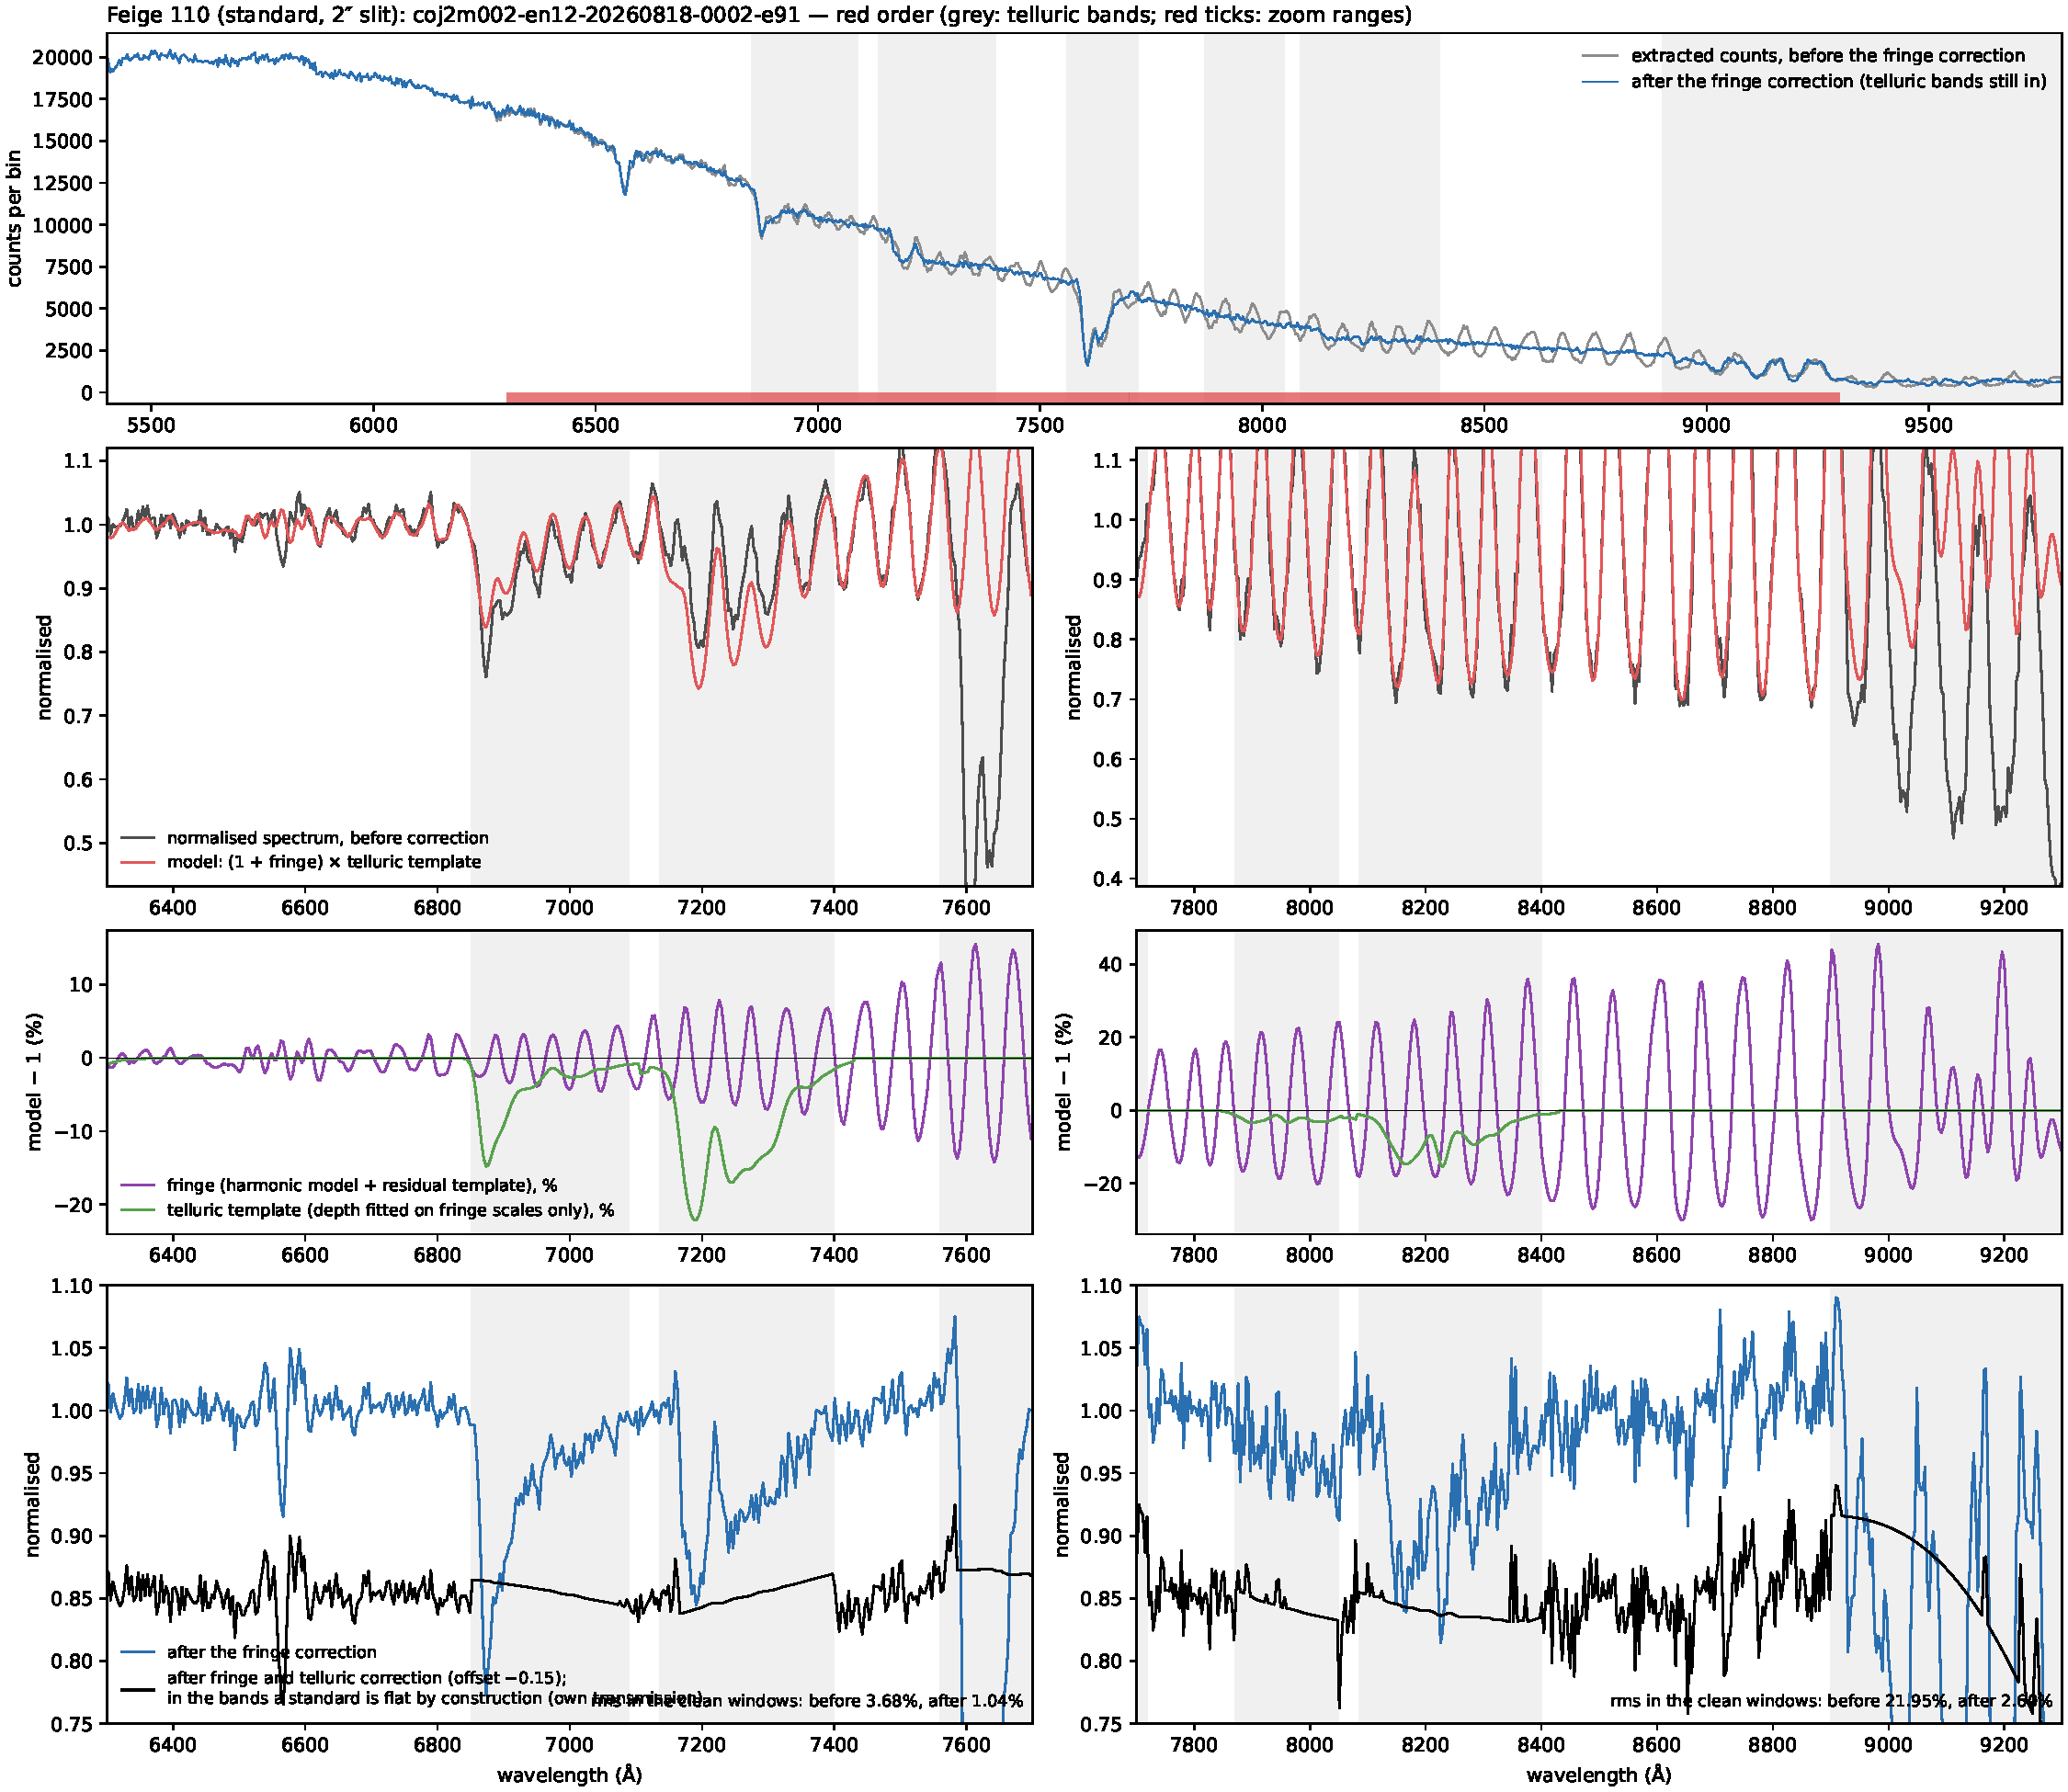
\includegraphics[width=\textwidth]{figures/fig_fringe_example_standard.pdf}
\caption{Fringe + telluric correction of the Feige\,110 exposure 2026-08-04 \#21 (fringe-fit residual 0.21; median of
the 39 exposures 0.26), at 6300--7700\,\AA{} (left) and 7700--9300\,\AA{} (right); grey shading: telluric bands. Top:
the normalised spectrum before correction (grey; counts over the reference at the FLOYDS resolution, over a smooth
continuum) and the fitted model. Middle: the same spectrum after the fringe and telluric correction (v3), with the
rms in the clean windows before $\to$ after. Bottom: the two model components, the fringe (including the residual
template of the slit) and the telluric template, whose depth is constrained only on fringe scales. Inside the bands
the corrected standard is smooth by construction, since its own transmission is measured there. The exposure with
the median residual can no longer be refitted (its 2-d pixel table was removed when the products were made lean,
Section~\ref{sec:sites_disk}); this is the nearest of the frames that keep it.}
\label{fig:fringe_example_std}
\end{figure}

\begin{figure}[!htbp]
\centering
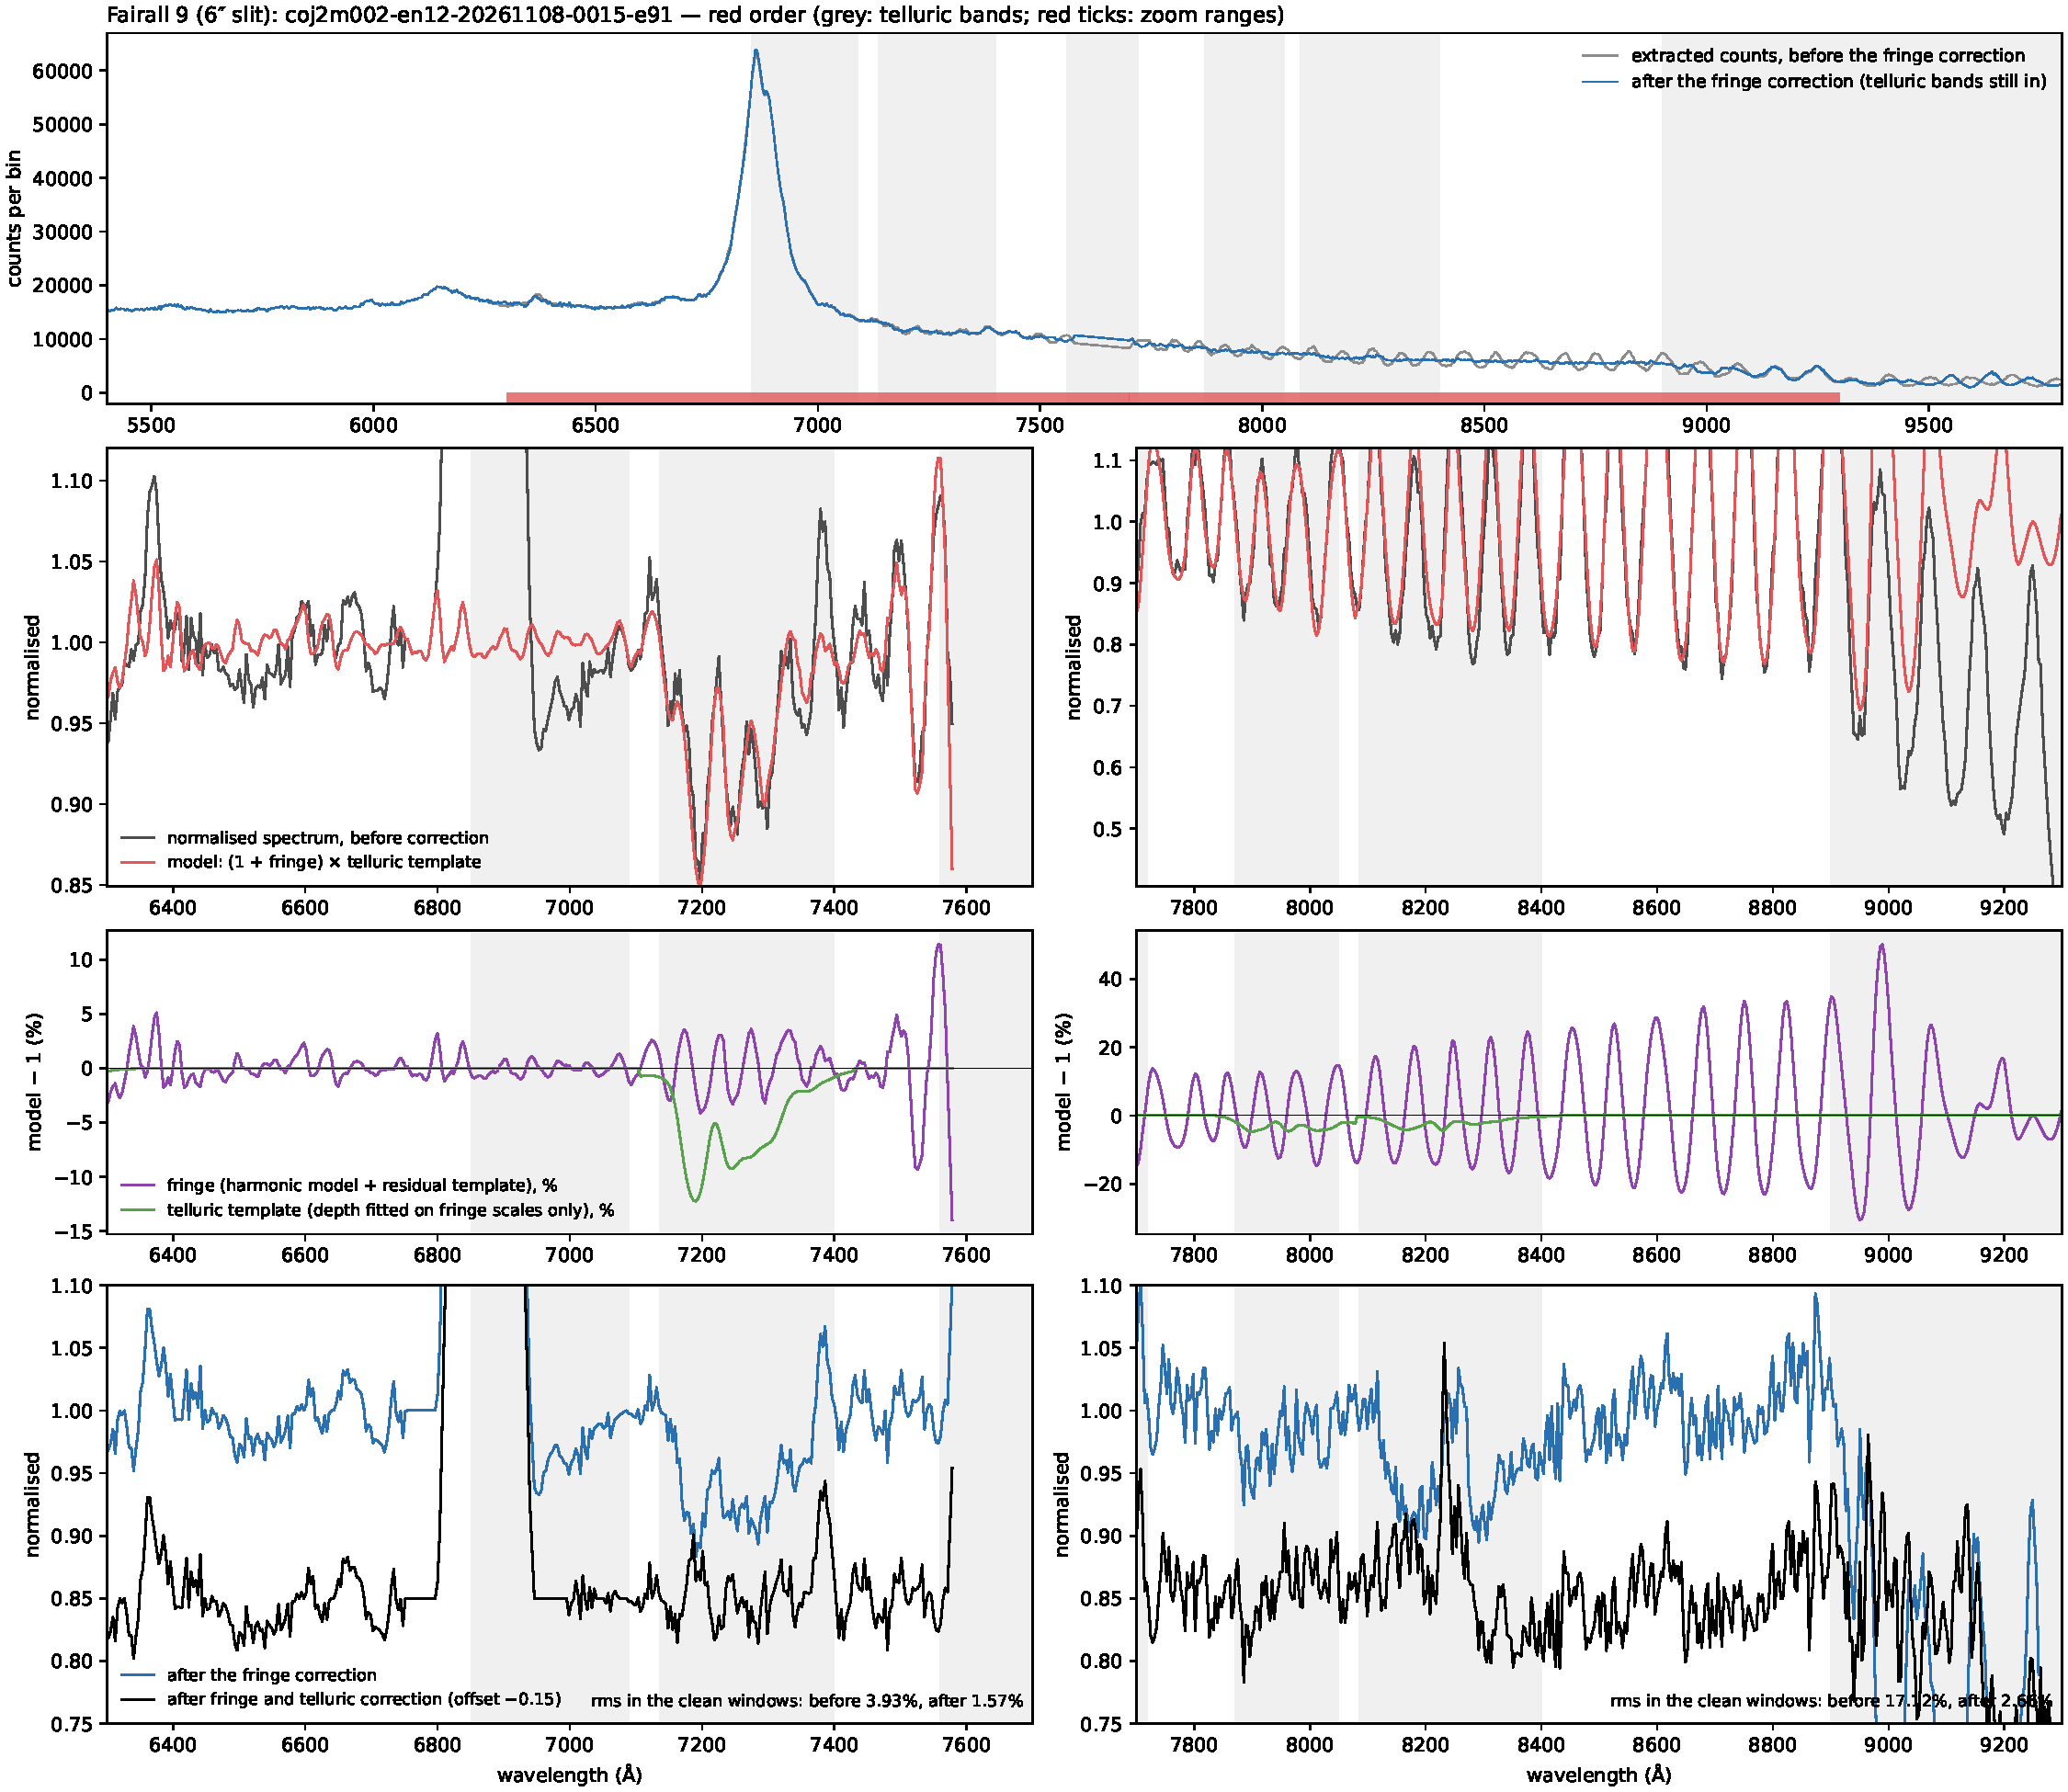
\includegraphics[width=\textwidth]{figures/fig_fringe_example_f9.pdf}
\caption{As Fig.~\ref{fig:fringe_example_std} for the Fairall~9 exposure 2026-08-28 \#9 (6\,arcsec slit), normalised
by a smooth continuum of the corrected spectrum (no reference: the AGN lines remain). The telluric correction of a
science frame is the median transmission of the nine nearest standards scaled to its airmass. Only two Fairall~9
frames keep the 2-d pixel table the refit needs; both are among the worst 5 per cent in the level of the
8110--8380\,\AA{} water band (this one ranks 96 of 100), which shows in the right-hand panels.}
\label{fig:fringe_example_f9}
\end{figure}

The 6300--7700\,\AA{} region is now inspected star by star in every assessment of the fringe correction
(Fig.~\ref{fig:zoom}, Section~\ref{sec:raw_compare}).
